% Architecture figure for README.md: tokens as communicating agents.
% Build (TeX Live 2025, from this directory):
%   pdflatex -interaction=nonstopmode agent_round.tex
%   pdftocairo -svg agent_round.pdf agent_round.svg
% The SVG carries glyphs as paths, so it renders identically on GitHub in every browser.
\documentclass[border=0pt]{standalone}
\usepackage[T1]{fontenc}
\usepackage{lmodern}
\usepackage{amsmath,amssymb}
\usepackage{tikz}
\usetikzlibrary{arrows.meta,positioning,fit,calc,backgrounds}

\definecolor{senderc}{RGB}{31,94,160}
\definecolor{receiverc}{RGB}{176,82,22}
\definecolor{channelc}{RGB}{90,90,90}

\pgfdeclarelayer{groups}
\pgfsetlayers{background,groups,main}

\begin{document}
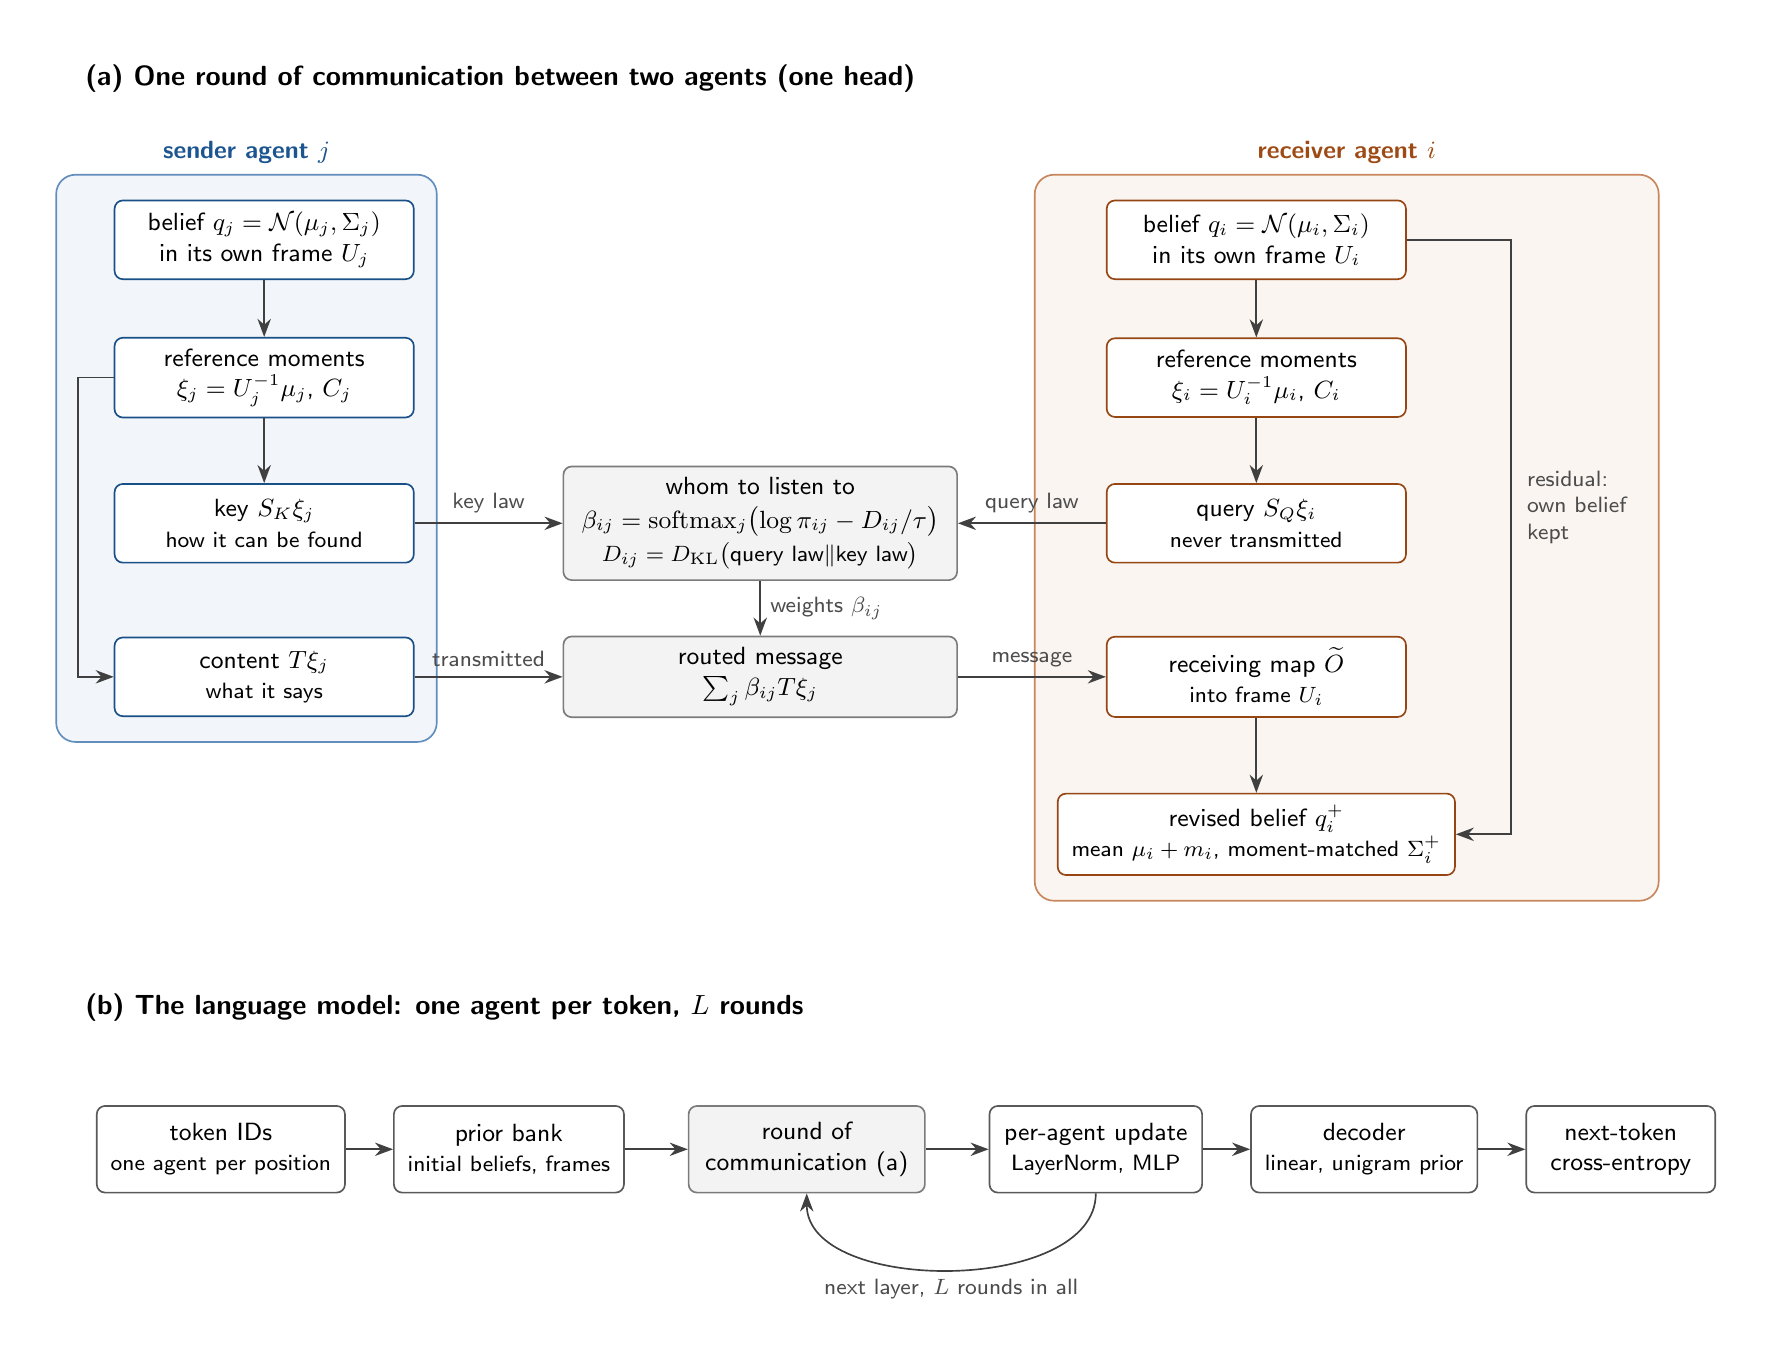
\begin{tikzpicture}[
    font=\sffamily\small,
    >={Stealth[length=2.3mm,width=1.7mm]},
    every path/.style={line width=0.6pt},
    box/.style={draw=black!65, rounded corners=3pt, fill=white, align=center,
                inner xsep=5pt, inner ysep=4pt, minimum width=38mm, minimum height=10mm},
    chan/.style={box, fill=channelc!7, draw=channelc!80},
    sbox/.style={box, draw=senderc!85!black},
    rbox/.style={box, draw=receiverc!85!black},
    flow/.style={->, draw=black!75},
    note/.style={font=\sffamily\footnotesize, text=black!70},
    panel/.style={font=\sffamily\bfseries, anchor=west},
    show background rectangle,
    background rectangle/.style={fill=white, rounded corners=6pt},
    inner frame sep=10pt,
]

% ---------------- Panel (a): one round of communication, one head ----------------
\node[panel] at (-2.4, 2.05) {(a) One round of communication between two agents (one head)};

% Sender agent j (left column)
\node[sbox] (sb)  at (0, 0)    {belief $q_j=\mathcal N(\mu_j,\Sigma_j)$\\ in its own frame $U_j$};
\node[sbox] (sxi) at (0, -1.75) {reference moments\\ $\xi_j=U_j^{-1}\mu_j$, $C_j$};
\node[sbox] (sk)  at (0, -3.6)  {key $S_K\xi_j$\\ \footnotesize how it can be found};
\node[sbox] (sc)  at (0, -5.55) {content $T\xi_j$\\ \footnotesize what it says};

% Receiver agent i (right column)
\node[rbox] (rb)  at (12.6, 0)    {belief $q_i=\mathcal N(\mu_i,\Sigma_i)$\\ in its own frame $U_i$};
\node[rbox] (rxi) at (12.6, -1.75) {reference moments\\ $\xi_i=U_i^{-1}\mu_i$, $C_i$};
\node[rbox] (rq)  at (12.6, -3.6)  {query $S_Q\xi_i$\\ \footnotesize never transmitted};
\node[rbox] (ro)  at (12.6, -5.55) {receiving map $\widetilde O$\\ \footnotesize into frame $U_i$};
\node[rbox] (rv)  at (12.6, -7.55) {revised belief $q_i^{+}$\\ \footnotesize mean $\mu_i+m_i$, moment-matched $\Sigma_i^{+}$};

% Channel (middle column)
\node[chan, minimum width=50mm] (route) at (6.3, -3.6)
    {whom to listen to\\[1pt]
     $\beta_{ij}=\mathrm{softmax}_j\bigl(\log\pi_{ij}-D_{ij}/\tau\bigr)$\\[1pt]
     \footnotesize $D_{ij}=D_{\mathrm{KL}}\bigl(\text{query law}\Vert\text{key law}\bigr)$};
\node[chan, minimum width=50mm] (pool) at (6.3, -5.55)
    {routed message\\ $\sum_j\beta_{ij}T\xi_j$};

% Path geometry kept inside the agent panels: the sender's content branch on the left, and the
% receiver's residual on the right, clear of the widest receiver box.
\coordinate (sleft) at ($(sxi.west)+(-0.45,0)$);
\coordinate (resx) at ($(rv.east)+(0.7,0)$);
\node[note, align=left, anchor=west] (reslab) at ($(rb.east -| resx)!0.45!(rv.east -| resx)+(0.08,0)$)
    {residual:\\ own belief\\ kept};

% Agent backgrounds
\begin{pgfonlayer}{groups}
  \node[fit=(sb)(sxi)(sk)(sc)(sleft), draw=senderc!70, fill=senderc!6, rounded corners=7pt,
        inner xsep=8pt, inner ysep=9pt, label={[text=senderc!90!black, font=\sffamily\bfseries\small]above:sender agent $j$}] (sender) {};
  \node[fit=(rb)(rxi)(rq)(ro)(rv)(resx)(reslab), draw=receiverc!70, fill=receiverc!6, rounded corners=7pt,
        inner xsep=8pt, inner ysep=9pt, label={[text=receiverc!90!black, font=\sffamily\bfseries\small]above:receiver agent $i$}] (receiver) {};
\end{pgfonlayer}

% Flows inside the agents
\draw[flow] (sb) -- (sxi);
\draw[flow] (sxi) -- (sk);
\draw[flow] (sxi.west) -- (sleft) |- (sc.west);
\draw[flow] (rb) -- (rxi);
\draw[flow] (rxi) -- (rq);
\draw[flow] (ro) -- (rv);
% Residual: the receiver keeps its own belief
\draw[flow] (rb.east) -- (rb.east -| resx) -- (rv.east -| resx) -- (rv.east);

% Flows through the channel
\draw[flow] (sk) -- node[note, above] {key law} (route);
\draw[flow] (rq) -- node[note, above] {query law} (route);
\draw[flow] (route) -- node[note, right] {weights $\beta_{ij}$} (pool);
\draw[flow] (sc) -- node[note, above] {transmitted} (pool);
\draw[flow] (pool) -- node[note, above] {message} (ro);

% ---------------- Panel (b): the model ----------------
\node[panel] at (-2.4, -9.75) {(b) The language model: one agent per token, $L$ rounds};

\begin{scope}[yshift=-11.55cm, box/.append style={minimum width=27mm, minimum height=11mm}]
  \node[box] (tok) at (-0.55, 0) {token IDs\\ \footnotesize one agent per position};
  \node[box, right=6mm of tok] (bank) {prior bank\\ \footnotesize initial beliefs, frames};
  \node[chan, minimum width=30mm, minimum height=11mm, right=8mm of bank] (round) {round of\\ communication (a)};
  \node[box, right=8mm of round] (mlp) {per-agent update\\ \footnotesize LayerNorm, MLP};
  \node[box, right=6mm of mlp] (dec) {decoder\\ \footnotesize linear, unigram prior};
  \node[box, right=6mm of dec, minimum width=24mm] (loss) {next-token\\ cross-entropy};
  \draw[flow] (tok) -- (bank);
  \draw[flow] (bank) -- (round);
  \draw[flow] (round) -- (mlp);
  \draw[flow] (mlp) -- (dec);
  \draw[flow] (dec) -- (loss);
  \draw[flow] (mlp.south) to[out=-90, in=-90, looseness=0.9] node[note, below] {next layer, $L$ rounds in all} (round.south);
\end{scope}

\end{tikzpicture}
\end{document}
